\documentclass[a4paper]{article}
\usepackage[T1]{fontenc}
\usepackage[utf8]{inputenc}
\usepackage{lmodern}
\usepackage[polish]{babel}
\usepackage{makeidx}
\usepackage{listings}
\usepackage{tabularx}
\usepackage{amsfonts}
\usepackage{graphicx}
\usepackage{hyperref}

\usepackage{listings}
\usepackage{alltt}

\usepackage[usenames,dvipsnames]{color}

\title{
	\textbf{ProtoDoc} v1.0 \\
	Google Protocol Buffers Documentation Tool\\ 
}
\author{
	Konrad Malawski \\
	konrad.malawski@java.pl \\
	\\ 
	Termin zajęć: Pon 9:45 \\
	EAIiE - Informatyka Stosowana, III Rok \\
	\\
	Data oddania projektu: 28 Czerwca 2011
}

\begin{document}

\maketitle

\newpage
\tableofcontents

\newpage

\section{Cel programu}
Celem projektu była wstępna implementacja narzędzia typu javadoc dla języka \textit{Google Protocol Buffers}.
Protocol Buffers, dalej zwane \textit{ProtoBuf}, jest to zbiór: języku definicji interfejsów, binarnego protokołu oraz rozszerzalnego kompilatora plików *.proto
do postaci kompilowalnych plików w dowolnym języku programowania, potrafiących przeczytać binarny strumień ProtoBuf tworząc z niego wygodne do użycia klasy dla programisty.
Z racji wysokiej wydajności parsowania tego typu \textit{Wiadomości} Protocol Buffers znajdują zastosowania w dużych systemach Enterprise, gdzie liczby wiadomości
osiągają rzędy setek lub tysięcy per system. Niestety nie jest możliwe w sposób czytelny dokumentować znaczenie poszczególnych pól lub wiadomości.

ProtoBuf jest odpowiedzią na tą potrzebę. Narzędzie to (napisane w całości w języku \textit{Scala}) umożliwia analogicznie jak JavaDoc, 
wygenerowanie dokumentacji projektu w postaci strony www na podstawie plików źródłowych oraz umieszczonych nad polami/wiadomościami komentarzami.

\section{Gramatyka Protocol Buffers IDL}
\subsection{Przykład pliku *.proto}
Celem unaocznienia gramatyki przytaczam tutaj przykład rzeczywistego pliku proto:
%\begin{verbatim}
\begin{lstlisting}
package pl.project13;

/** sample comment */
message FormMessage {

    /** sample comment */
    enum ContactVia {
        SMS = 1;
        PHONE = 2;
    }

    /** sample comment */
    required ContactVia contact_me_via = 1;

    optional string name = 2 [default = "loremipsum"];

    /** sample comment */
    message InnerMessage {
        /** sample comment */
        required string name = 3;
        required string surname = 4;
        optional string age = 5;
    }
} 
\end{lstlisting}
%\end{verbatim}


 
\subsection{Gramatyka języka Protocol Buffers IDL}
\subsubsection{Tabela tokenów}
\begin{center}
\begin{tabular}{| l | l | p{5cm} | p{5cm} |}
\hline
\textbf{L.p.} &  \textbf{Nazwa Tokena}            & \textbf{Opis}                                 & \textbf{Komentarz} \\ \hline
1    & \verb`newLine`          & \verb`\r | \n | \r\n`                & Znak nowej linii, na różnych systemach \\ \hline
2    & \verb`endOfLine`               & \verb`\n`                            & Rzeczywista nowa linia \\ \hline
3    & \verb`whiteSpace`       & \verb`" " | \t | \f | {NEW_LINE}`    & Biały znak \\ \hline
7    & \verb`commentLine`       & \verb`"/""/"[^\r\n]*/`                & C-Style Komentarz \\ \hline
8    & \verb`intLit`            & \verb`decInt | hexInt | octInt`      & Liczba całkowita \\ \hline
9    & \verb`decLit`            & \verb`/[1-9]\d*/`                    & Liczba w zapisie dziesiętnym \\ \hline
11   & \verb`hexLit`            & \verb`/0[xX]([A-Fa-f0-9])+/`         & Liczba w zapisie heksadecymalnym \\ \hline
11   & \verb`octLit`            & \verb`/0[0-7]+/`                     & Liczba w zapisie ósemkowym \\ \hline
10   & \verb`strLit`            & \verb`quote (hexEscape | octEscape`
                                  \verb`| charEscape | /[^\0\n]/)*`
                                  \verb`quote`                         & Ciąg znaków \\ \hline
11   & \verb`floatLit`          & \verb`/\d+(\.\d+)?([Ee][\+-]?\d+)?/` & Liczba zmienno przecinkowa \\ \hline
11   & \verb`boolLit`           & \verb`true|false`                    & Wartość booleanowa \\ \hline
11   & \verb`quote`             & \verb`/["']/`                        & Rozpoczęcie lub zakończenie ciągu znaków \\ \hline
15   & \verb`ident`             & \verb`/[A-Za-z_][\w_]*/`                &  Identyfikator \\ \hline

16   & \verb`coma`              & \verb`,`                &  Przecinek \\ \hline
17   & \verb`equal`             & \verb`=`                &  Przypisanie \\ \hline
18   & \verb`semiColon`         & \verb`;`                &  Średnik, koniec linii kodu \\ \hline
19   & \verb`openBlock`        & \verb`{`                &  Otwarcie bloku kodu \\ \hline
20   & \verb`closeBlock`       & \verb`}`                &  Zamknięcie bloku kodu \\ \hline
21   & \verb`openBrace`        & \verb`[`                &  Otwarcie inicjalizatora \\ \hline
22   & \verb`closeBrace`       & \verb`]`                &  Zamknięcie inicjalizatora \\ \hline
23   & \verb`openParant`       & \verb`(`                &  Otwarcie nawiasu \\ \hline
24   & \verb`closeParant`      & \verb`)`                &  Otwarcie nawiasu \\ \hline
32   & \verb`hexEscape`        & \verb`/\\[Xx][A-Fa-f0-9]{1,2}/` & Escape'owana liczba hexadecymalna \\ \hline
33   & \verb`octEscape`        & \verb`/\\0?[0-7]{1,3}/` & Escape'owana liczba ósemkowa \\ \hline
34   & \verb`charEscape`       & \verb`/\\[abfnrtv\\\?'"]/` & Escape'owany znak \\ \hline

% indentyfikatory
  & \verb`enum` & \verb`enum` & Enumeracja \\ \hline
  & \verb`package` & \verb`package` & Paczka \\ \hline
  & \verb`message` & \verb`message` & Wiadomość \\ \hline
\end{tabular}
\end{center}

\newpage

\begin{center}
\begin{tabular}{| l | l | p{5cm} | p{5cm} |}
\hline
\textbf{L.p.} &  \textbf{Nazwa Tokena}            & \textbf{Opis}                                 & \textbf{Komentarz} \\ \hline
  & \verb`repeated` & \verb`repeated` & Pole powtarzane \\ \hline
  & \verb`optional` & \verb`optional` & Pole opcjonalne \\ \hline
  & \verb`required` & \verb`required` & Pole wymagane \\ \hline
  & \verb`true` & \verb`true` & \\ \hline
  & \verb`false` & \verb`false` & \\ \hline
  & \verb`camelLit` & \verb`/[A-Z][A-Za-z_]*/` & \\ \hline
  & \verb`int32` & \verb`int32` & \\ \hline
  & \verb`uint32` & \verb`int32` & \\ \hline
  & \verb`int64` & \verb`int64` & \\ \hline
  & \verb`uint64` & \verb`uint64` & \\ \hline
  & \verb`bytes` & \verb`bytes` & \\ \hline
  & \verb`float` & \verb`float` & \\ \hline
  & \verb`double` & \verb`double` & \\ \hline
  & \verb`sint32` & \verb`sint32` & Typ całkowity, ze znakiem, 32 bitowy \\ \hline
  & \verb`sint64` & \verb`sint64` & Typ całkowity, ze znakiem, 64 bitowy \\ \hline
  & \verb`fixed32` & \verb`fixed32` & Typ \\ \hline
  & \verb`fixed64` & \verb`fixed64` & Typ \\ \hline
  & \verb`sfixed32` & \verb`sfixed32` & Typ \\ \hline
  & \verb`sfixed64` & \verb`sfixed64` & Typ \\ \hline
  & \verb`bool` & \verb`bool` & Typ \\ \hline
  & \verb`string` & \verb`string` & Typ \\ \hline
  & \verb`bytes` & \verb`bytes` & Typ \\ \hline
  & \verb`userType` & \verb`/\.? ident (\. ident)* /` & Typ \\ \hline
\end{tabular}
\end{center}

\subsubsection{Gramatyka}
\begin{verbatim}
proto : ( message | enum | package | ";" )*

package : "package" ident ( "." ident )* ";"

message : "message" ident messageBody

enum : "enum" ident "{" ( option | enumField | ";" )* "}"

enumField : ident "=" intLit ";"

messageBody : "{" ( field | enum | message | ":" )* "}"

# tag number must be 2^29-1 or lower, not 0, and not 19000-19999 (reserved)
field : label type ident "=" intLit ( "[" fieldOption ( "," fieldOption )* "]" )? ";"

fieldOption : "default" "=" constant

label : "required" | "optional" | "repeated"

type : "double" | "float" | "int32" | "int64" | "uint32" | "uint64"
       | "sint32" | "sint64" | "fixed32" | "fixed64" | "sfixed32" | "sfixed64"
       | "bool" | "string" | "bytes" | userType

# leading dot for identifiers means they're fully qualified
userType : "."? ident ( "." ident )*

constant : ident | intLit | floatLit | strLit | boolLit
\end{verbatim}


\section{Opis i schemat struktury logicznej programu}
Program korzysta z \textit{Scala ParserCombinators}, części biblioteki \textbf{będącej częścią tego języka} przeznaczonej właśnie genrowaniu parserów.
Wykorzystanie \textit{ParserCombinators} nad inne znane rozwiązania typu JBison/JFlex i im podobne (JACC (odpowiednik Javowy narzędzia YACC)) motywuję
niesamowitym potencjałem języka Scala oraz możliwości wprost programowania oraz wpinania się w nasz odeclowy model obiektowy domeny podczas parsowania.
Takie podejście nie byłoby możliwe przy zastosowaniu klasycznych 'compiler compiler'ów.

Pierwszym krokiem jest przeparsowanie pliku proto przez zaimplementowany dla tego projektu kombinator parserów. Krok ten wykonywany 
jest dla każdego z plików jaki zostanie odnaleziony na ścieżce wejściowej podanej aplikacji. Pierwotnie nie była przewidywana obsłuwa wielu 
plików na tym etapie ProtoDoc, jednak implementacja okazała się dzięki Scali bardzo wygodna i sprawna. Po przeparsowaniu wszystkich plików, 
otrzymujemy listę wiadomości zawierających \textit{kompletną} strukturę pól oraz wiadomości lub enumeracji zagnieżdżonych w tych typach. 
Zachowana zostaje również poprawność ścieżek package do wiadomości wewnętrznych - wówczas \textit{package} sub-wiadomości powinien zawierać (kończyć się na) 
\textit{message} w którym się zawiera.

Kolejnym krokiem jest generowanie na podstawie listy wiadomości stron HTML zawierających dokumentację. Dzięki pelnej reprezentacji wszystkich elementów 
przeparsowanych plików - w tym komentarzy oraz zagnieżdżeń typów w typach proces ten jest stosunkowo prosty i odbywa się przy pomocy zastosowaniu
kilku funkcyjnych metod/własności kolekcji języka Scala, konkretniej: map, reduce, fold, oraz filter. Przy pomocy złożeń tych transformacji kolekcji bardzo łatwo było
uzyskać na przykład listę wszystkich typów, które następnie transformowano na wspólny im nad typ, aby przekazać do systemu szablonowego.  
Jest to o tyle ciekawe oraz istotne iż w każdym kroku tego procesu zachowywane są całe struktury obiektów jak i ich typy. W żadnym miejscu programu nie mamy 
do czynienia z operowaniem na jedynie napisach - gdyż tak byłoby w wielu językach o wiele łatwiej filtrować tylko interesujące nas wiadomości; dzięki \textit{Scala}
praca na rzeczywistych typach nie tylko była wygodna, ale również naturalna.

\newpage
Wybrany do implementacji warstwy widoku język szablonów nazywa się "\textit{Mustache}". Jego nazwa pochodzi od składni jaką się posługuje wypisując zmienne w szablonach
\textit{mustache}. Poniżej mały przykłąd prostego szablonu \textit{mustache}:
\begin{verbatim}
 <ul>
   {{#fields}}
     <li>name: {{name}}</li>
   {{/fields}}
 </ul>
\end{verbatim}
Proces generowanie ProtoDoc kończy się w momencie przekazania ostatniej wiadomości (lub enumeracji) do systemu szablonów. 
Wynikowe pliki HTML są zapisywane do podanego podczas uruchamiania aplikacji przez użytkownika folderu. 

Przeglądanie stron jest możliwe zarówno przy wykorzystaniu przeglądarek obsługujących JavaScript -- wówczas dostępna jest wyszukiwarka jak i nawigacja 
,,na jednej stronie'' z zachowaniem historii, oraz przy wykorzystaniu przeglądarek tekstowych (takich jak links). W przypadku przeglądania strony w trybie tekstowym,
wyświetlana jest bardzo czytelna dla takich przeglądarek stron wersja, która oczywiście nie wymaga do działania obsłgi \textit{JavaScript}u. 


\section{Wykorzystane pakiety zewnętrznye i narzędzia}
Poniżej wymieniono zależności projektu wykorzystane celem implementacji jak i testowania tego projektu.

\begin{itemize}
 \item \textbf{Scala} --- sam język w którym zaimplementowano to rozwiązanie jest wart wymienienia 
                        jako najważniejsze narzędzie w tym projekcie. Jest on niebywałym połączeniem języków funkcyjnych (takich jak LISP czy Haskell)
                        oraz klasycznych (w sensie 'znanych nam') zorientowanych stricte obiektowo, vide Java. Scala jest językiem statycznie typowanym,
                        jednak posiada o wiele bardziej rozbudowany system inferowania typu niż inne obecnie popularne języki na rynku informatycznym,
                        właściwość ta niejednokrotnie przydała się podczas implementowania parsera, gdzie łatwo było napisać 'implicite' konwersje między pewnymi typami.
                        Same ParserCombinators oczywiście również zasługują na wspomnienie, są bowiem częścią biblioteki standardowej Scala i dzięki nim projekt ten stał się \textit{czystą przyjemnością}.
 \item \textbf{Scalate} oraz \textbf{Mustache} --- Scalate został wykorzystany jako silnik szablonów celem renderowania wynikowych stron HTML z dokumentacją ProtoBuf.
                                                   Mustache jest jednym z kilku implementowanych przez Scalate języków szablonów. Mustache wyróżnia się tym spośród innych
                                                   iż zupełnie nie posiada logiki - dzięki temu logika biznesowa (bądź wszelakiego rodzaju filtrowania kolekcji etc)
                                                   nie przeciekną nam do wartwy widoku. Dzięki niemu testowanie widoku oraz rozwój aplikacji włącznie ze zmianami reprezentacji
                                                   pewnych typów przed przekazaniem ich do szablonu były bardzo wygodne.
 \item \textbf{sbt} (Simple Build Tool) -- jest to odpowiednik Maven lub Ant znanych ze świata Javowego jednak dla języka Scala. Możliwe jest również kompilowanie
                                           przy jego pomocy projektów Java jednak nie jest to raczej spotykane. Dzięki łatwości konfiguracji zadań sbt w przeciwieństwie
                                           do dodawania własnych pluginów do systemu Maven okazał się wysoce pomocny podczas budowania wykonywalnego pliku jar z protodoc.
                                           Najważniejszą cechą \textbf{sbt} która okazała się wysoce pomocna podczas tego projektu jest możliwość odpalania testów w trybie ciągłym,
                                           dzięki czemu zawsze (co każdą zmianę w pliku źródłowym) mamy informację zwrotną jaki wpływ ta zmiana miała na testy - metoda
                                           ta w połaczeniu z metodyką TDD okazała się wysoce efektywna i przyjemna podczas rozwoju oraz poprawiania usterek w aplikacji.
 \item \textbf{ScalaTest} -- Prosty framework służący pisaniu testów jednostkowych w języku Scala.
                             Można go potraktować jako odpowiednik JUnit (znany z świata Javowego) jednak odrobinę potężniejszy - dzięki przewadze semantycznej języka Scala.
\end{itemize}


\newpage
\section{Informacje o zastosowaniu specyficznych metod rozwiązania problemu}
Specyficznym rozwiązaniem w samym parserze są \textit{Scala ParserCombinators} - część języka dedykowana budowaniu Parserów, przy pomocy przeznaczonego
temu DSLa (Domain Specific Language), choć nadal pozostając z ,,czystej Scala''. Jedną z zalet zastosowania tego narzędzia nad innymi jest 
brak kolejnego procesu kompilacji który zazwyczajbyśmy musieli zastosować - na przykład wykorzystując Flex/Bisona lub inne rozwiązania którymi
,,klasycznie'' generuje się parsery. 

ParserCombinators wywodzą się z bardzo ciekawego pomysłu, jak sama nazwa wskazuje, kombinowania parserów. Dzięki temu poniższy, poprawny w języku Scala,
zapis: 

\begin{verbatim}
 def boolValue = ("true" | "false")
\end{verbatim}

Definiuje w sumie 3 parsery:
\begin{itemize}
 \item parser wyrażenia ,,true'', zwracający wartość jako \textit{java.lang.String} (gwarantują to właściwości typów języka \textit{Scala})
 \item parser wyrażenia ,,false'', zwracający wartość jako \textit{java.lang.String} (gwarantują to właściwości typów języka \textit{Scala})
 \item parser \textbf{alternatywa}, dwóch wcześniej zdefiniowanych parserów. 
\end{itemize}
Dzięki takiej kombinacji parserów, osiągamy bardzo czytelną składnię do definiowania naszego języka oraz bardzo potężne narzędzie w postaci 
możliwości ,,wpięcia się'' w dowolny moment parsowania zwyczajnym kodem \textit{Scala} i przetworzenia na przykład wybranego typu, na wartość
innego typu. Idąc tym tokiem rozumowania możemy rozbudować nasz boolValue parser aby zwracał wartość \textbf{Boolean} zamiast \textbf{String}.

Dokonamy tego dzięki zastosowaniu kolejnego kombinatora, o nazwie \textit{,,function applying combinator''} oraz oznaczeniu: \verb|^^|.
Kombinator ten dokonuje transformacji kombinatora parserów po jego lewej stronie, przy pomocy funkcji przekazanej jego prawej stronie.
W języku Scala przekazywanie funkcji wyższego rzędu jest dość trywialne, zatem nasz problem transformacji \textbf{String}a na \textbf{Boolean} 
rozwiązalibyśmy następująco:

\begin{verbatim}
 def boolValue = ("true" | "false") ^^ {
   s =>
     s.toBoolean
 }
\end{verbatim}

Pamiętamy nadal iż typ kombinatora parserów na którym pracujemy tą funkcją (przekazany jako parametr funkcji anonimowej - \textbf{s})
to \textit{java.lang.String}. Przypominamy sobie iż klasyczny String nie posiada przecież metody \textbf{toBoolean()} (w \textit{Scala} dozwolone jest 
pomijanie nawiasów okrągłych, stąd \textbf{toBoolean} oznacza wywołanie metody \textbf{toBoolean()}). Poznaliśmy właśnie kolejną możliwość języka Scala.

Istnieją tak zwane konwersje \textbf{\textit{implicit}}, dzięki którym ,,jeżeli wygląda na to iż potrzebujemy skonwertować jeden typ na inny'' zostanie zastosowana
konwersja implicit, i uzyskamy pożądany typ. W powyższym przykładzie zadziałało to na zasadzie, istniejącej w bibliotece standardowej konwersji \textit{implicit}:

\begin{verbatim}
 implicit def string2richString(str: String) = new RichString(str)
\end{verbatim}

Dzięki tej konwersji otrzymaliśmy obiekt RichString, na którym zostanie zawołana metoda toBoolean (\url{http://www.scala-lang.org/api/2.7.4/scala/runtime/RichString.html#toBoolean}).
Zwracany typ tej metody to \textbf{scala.Boolean}. Ostatnim krokiem utworzenia tego kombinatora jest kolejna konwersja \textit{implicit} która zostanie 
wywołana w momencie zwrócenia naszej funkcji anonimowej. Podczas gdy zwróciliśmy typ scala.Boolean (słowo kluczowe "\textbf{return}" jest w tym przypadku opcjonalne),
def boolValue powinno być \textbf{Parser}em, dzięki kolejnej implicit konwersji ostatecznie boolValue otrzyma typ Parser[Boolean] i gdy będziemy chcieli pobrać wartość 
tym sposobem przeparsowanego Tokena, otrzymamy wartość typu \textbf{scala.Boolean}. 

Jak łatwo się domyślić, przedstawione mechanizmy do dopiero czubek góry lodowej jaką jest język \textbf{Scala} i \textbf{ParserCombinators}.
Uważam, że praca z tak zaawansowanym językiem jak i DSLem do definiowania parserów gramatyk jest niebywale interesującym oraz pouczającym przeżyciem.

Ponad to, otrzymany w efekcie kod Parsera do złudzenia przypomina gramatykę EBNF, a więc jest bardzo czytelna oraz łatwa w implementacji oraz dalszym rozwoju.
Przed wyborem tego narzędzia testowałem klasyczne podejścia do problemu przy pomocy JFlex/JBison jednak nie były to tak przyjemne w użyciu oraz rozwoju narzędzia 
jak czysty język Scala i jego funkcyjna natura.



\newpage
\section{Instrukcja obsługi}
\subsection{Pobranie aktualnych źródeł}
Aby pobrać najświeższą wersję źródeł należy skorzystać z systemu wersjonowania \textbf{git}:
\begin{verbatim}
 git clone git://github.com/ktoso/protodoc-scala.git
 cd protodoc-scala
\end{verbatim}

\subsection{Uruchomienie aplikacji przez sbt}
Następnie do uruchomienia aplikacji (bądź jej skompilowania) o skompilowania można wykorzystać poniższy ciąg poleceń.
Zakładamy iż użytkownik posiada zainstalowany w systemie \textbf{sbt} - Simple Build Tool, najpopularniejsze narzędzie budowania 
projektów w języku Scala (obsługuje również projekty w Java, z domyślnym layotem \textbf{Maven}owym).

Aby uruchomić aplikację:
\begin{verbatim}
 sbt run [parametry aplikacji]
\end{verbatim}

W przypadku nie podania wymaganych parametrów do uruchomienia ProtoDoc, zostaniemy o tym poinformowani następującą wiadomością:
\begin{verbatim}
usage: ProtoDoc [options] proto_dir out_dir

options:
  -v, --verbose   active verbose output, [default = false]
  --------------------------------------------------
  proto_dir       directory containing proto files to parse
  out_dir         output directory for the protodoc html webpage
\end{verbatim}

Zatem poprawne wywołanie aplikacji wyglądałoby następująco: 
\begin{alltt}
 sbt run ~/coding/protodoc-scala/src/main/proto/simple /tmp

 # kompilacja aplikacji

[info] == run ==
[info] Running pl.project13.protodoc.runner.ProtoDocMain 
                        ~/coding/protodoc-scala/src/main/proto/simple /tmp
verbose: false
proto_dir: ~/coding/protodoc-scala/src/main/proto/simple
out_dir: /tmp
Parsing file: ~/coding/protodoc-scala/src/main/proto/simple/simple.proto
Parsing file: ~/coding/protodoc-scala/src/main/proto/simple/multiple_inner_msgs.proto
Parsing file: ~/coding/protodoc-scala/src/main/proto/simple/amazing_message.proto
Parsing file: ~/coding/protodoc-scala/src/main/proto/simple/with_enum.proto
Message: \textbf{pl.project13.WithEnum}
Message: \textbf{pl.project13.AmazingMessage}
Inner:   pl.project13.AmazingMessage.\textbf{InnerMessage}
Message: \textbf{pl.project13.TopLevel}
Inner:   pl.project13.TopLevel.\textbf{MiddleLevel}
Inner:   pl.project13.TopLevel.MiddleLevel.\textbf{InnerInnerLevel}
Message: \textbf{pl.project13.MessageWithInner}
Inner:   pl.project13.MessageWithInner.\textbf{InnerMessage}
[info] == run ==
[success] \textcolor{OliveGreen}{Successful.}
\end{alltt}

Możliwe jest również przekazanie opcji \textit{-v}, która skutkuje znacznym zwiększeniem stopnia logowanych na konsolę wiadomości.
Raczej powinna być ona zbędna użytkownikowi, pozostawiono ją dostępną jednak na wypadek potrzeby debugowania aplikacji 'wizualnie'.

W razie potrzeby możliwe jest również wygenerowanie pliku wykonywalnego JAR, aby tego dokonać należy skorzysać z dwóch poleceń sbt:
\begin{verbatim}
 sbt collect-jars
 sbt package
\end{verbatim}
Plik znajdzie się w folderze \textbf{target/scala-2.8.1} (ponieważ pod tą wersję Scala projekt został właśnie skompilowany).

\subsection{Z pliku JAR}
Udostępniona została również skompilowana paczka tej aplikacji, można ją poprać z:
\begin{verbatim}
 wget http://up.project13.pl/protodoc/protodoc-1.0.tar.gz
\end{verbatim}
A następnie wykonać w następujący sposób:
\begin{verbatim}
 tar xzvf protodoc-1.0.tar.gz
 java -jar protodoc-1.0.jar [parametry aplikacji]
\end{verbatim}

\subsection{Przy wykorzystaniu aplikacji protodoc-gui}
Dla tego projektu powstała również malutka aplikacja pozwalająca możliwie najłatwiej testować parser ręcznie.
Aplikację można uruchomić poprzez przejście do jej folderu oraz uruchomienie polecenia: 
\begin{verbatim}
 git clone git://github.com/ktoso/protodoc-gui.git
 ant run
\end{verbatim}
Zakładamy iż ścieżki do bibliotek zostały ustalone poprawnie przez użytkownika oraz iż posiada zainstalowane na swoim systemie narzędzie \textbf{ant}.

Aplikacja ta pozwala na edycję definicji Protocol Buffers po lewej stronie aplikacji oraz skompilowanie jej w miejscu. Kompilacja definicji tworzonej po lewej 
stronie jest automatycznie właczana co zmianę w źródle. Dzięki temu można na żywo śledzić jak zachowuje się parser podczas powstawania kolejnych fragmentów definicji interfejsu.

\newpage
\begin{figure}[ch!]
 \centering
 \includegraphics[width=30em]{protodoc_gui}
 \caption{Screenshot GUI ułatwiającego manualne testowanie aplikacji}
 \label{fig:gui}
\end{figure}



\newpage
\section{Przykładowe wyniki działania programu}
\subsection{Wynikowa strona www ProtoDoc}
Z przykładowych plików *.proto, umieszczonych w folderze projektu 'src/main/proto/simple' 
zostanie wygenerowana strona ProtoDoc o wyglądzie przedstawionym na załączonych zrzutach ekranu.
W obecnej wersji aplikacji generowane są widoki Message (wiadomości - vide Rysunek \ref{fig:protodoc_msg}), Enum (enumeracji - vide Rysunek \ref{fig:protodoc_enum}) 
oraz ogólny widok index.html (vide Rysunek \ref{fig:protodoc_main}) zawierający również spis wszystkich Typów dostępnych w analizowanym folderze. Dostępna jest również wyszukiwarka, filtrująca tę listę na podstawie 
wpisanego fragmentu nazwy.

\begin{figure}[ch!]
 \centering
 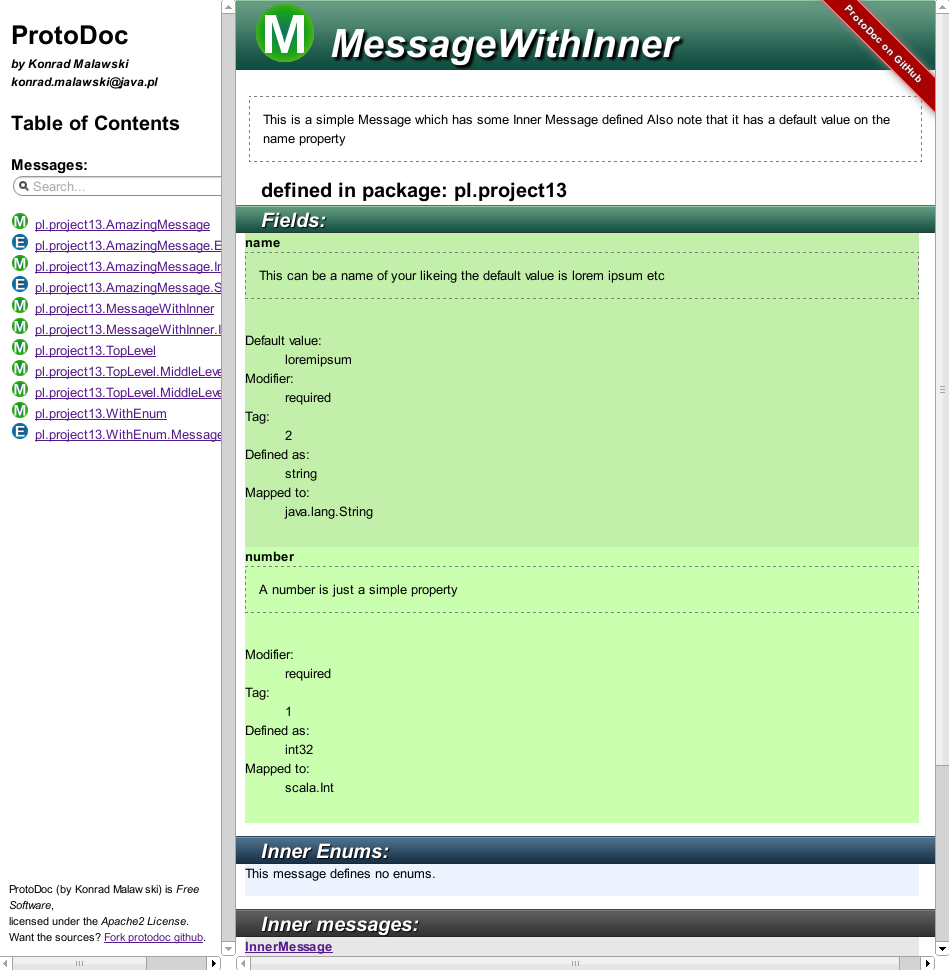
\includegraphics[width=35em]{protodoc_main}
 \caption{Główny widok ProtoDoc}
 \label{fig:protodoc_main}
\end{figure}
\begin{figure}[ch!]
 \centering
 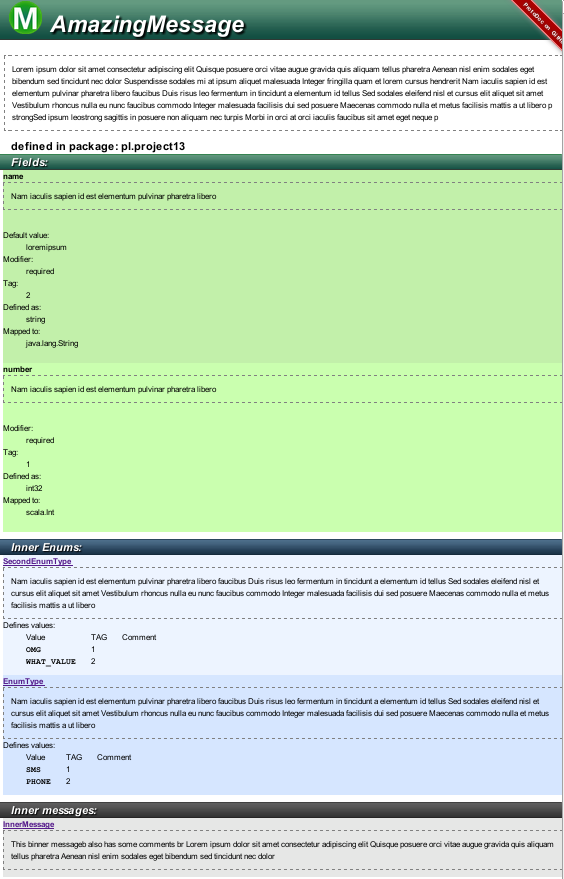
\includegraphics[width=35em]{protodoc_msg}
 \caption{Widok dokumentacji wiadomości}
 \label{fig:protodoc_msg}
\end{figure}
\begin{figure}[ch!]
 \centering
 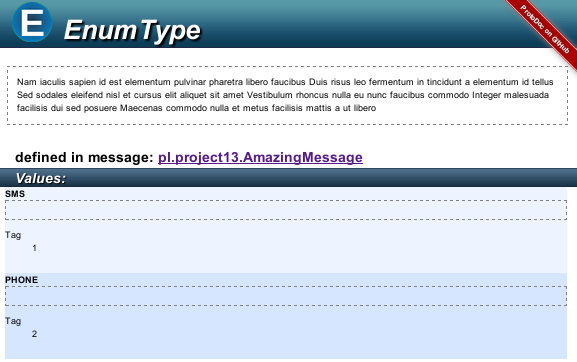
\includegraphics[width=35em]{protodoc_enum}
 \caption{Widok dokumentacji enumeracji (enum)}
 \label{fig:protodoc_enum}
\end{figure}

\newpage
\subsection{Przykłady wykrywanych błędów}
ProtoDoc w obecnej wersji potrafi już wykrywać niektóre rodzaje błędów jakie może napotkać w plikach źródłowych.
Poniżej zostaną przedstawione niektóre z nich. Poza przedstawionymi tutaj mechanizmami typowe ,,nie pasowanie do gramatyki''  
na przykład poprzez definicję enumeracji jako ,,top level'' jednostki również zostanie zgłoszone w analogiczny sposób. 
Każdy z tych składniowych niesie ze sobą informację o miejscu gdzie błąd wystąpił (w postaci numeru linii i kolumny), 
wraz dotyczącym błędu fragmentem kodu oraz wskazaniem znakiem \textbf{\^} miejsca wystąpienia problemu.

\subsubsection{Wykrycie niepoprawnego modyfikatora}
Poniższa wiadomość zawierająca błąd w słowie ,,optional'', będącym modifykatorem pola ProtoBuf.
\begin{verbatim}
message Msg {
zoptional int32 number = 12;
}
\end{verbatim}

wywoła komunikat błędu:
\begin{alltt}
\textcolor{Red}{pl.project13.protodoc.exceptions.ProtoDocParsingException: 
\textbf{[2.1]} failure: `\}' expected but `' found 

zoptional int32 costam = 23;
\textbf{\^} }
\end{alltt}
Warto zauważyć znak \textbf{\^} oznaczający dokładnie miejsce wystąpienia problemu, ponad to zwracana jest pozycja problemu, w postaci objętych
kwadratowymi nawiasami numeru wiersza oraz numeru kolumny gdzie problem wystąpił.

\subsubsection{Wykrycie zastosowanie nie zdefiniowanego typu}
Poniższa definicja zawiera odwołanie do niezdefiniowanego typu - UnknownType. ProtoDoc jest w stanie wykryć ten problem oraz zareaguje 
rzuceniem wyjatku typu ,,\textit{pl.project13.protodoc.exceptions.UnknownTypeException}'' podając również przyczynę problemu.
\begin{verbatim}
message Msg {
required UnknownType field = 23;
} 
\end{verbatim}
spowoduje rzucenie następującego komunikatu:
\begin{alltt}
\textcolor{Red}{pl.project13.protodoc.exceptions.UnknownTypeException: 
Unable to link '\textbf{UnknownType}' to any known enum Type.}
\end{alltt}

\subsubsection{Wykrycie nie zdefiniowanej opcji}
Program jest gotowy do dalszego rozwoju w kierunku deklarowania własnych Opcji. Jest to funkcja dokumentowana przez Google jako 
najprawdopodobniej nie potrzebna 98 procent użytkowników Protocol Buffers jednak jako, że dokładnie przez opcje jest zdefiniowana wartość domyślna pola,
po niekąd część funkcjonalności (rozpoznawanie) ich została już zaimplementowana w tej wersji ProtoDoc. Poniżej przykład nie odnalezienia pasującej opcji na polu \textit{field}.

\begin{verbatim}
message Msg {
  required string field = 1 [default = VALUE];
  required uint64 field = 2 [def = VALUE];
} 
\end{verbatim}
Spowoduje to wypisanie następującego komunikatu błędu:

\begin{alltt}
\textcolor{Red}{pl.project13.protodoc.exceptions.ProtoDocParsingException: 
[3.30] failure: `default' expected but `d' found

  required uint64 field = 2 [def = VALUE];

                             ^}\end{alltt}

Jak widać, opcja \textbf{def} nie została odnaleziona spośród rozpoznawanych opcji (zbiór jedynie opcji \textbf{default},
i został rzucony wyjątek ProtoDocParsingException.

\newpage
\subsection{Przykład możliwie zaawansowanej wiadomości rozpoznawanej na tym etapie przez ProtoDoc}
Poniżej przykład wiadomości wykorzystujący wszystkie zaimplementowane możliwości parsera oraz generatora będących częścią ProtoDoc v1.0.

\begin{verbatim}
package pl.project13.protodoc;

message Msg {

  enum KnownType {
    VALUE = 1;
    OTHER = 2;
  }
  
  /** This is an inner message */
  message InnerMsg {
    enum InnerEnum {  }

    /** Infinite embeddability */
    message InnerInnerMsg {  }

    required double dNumber = 1;    
    optional float fNumber = 2;    
  }

  required string field = 1 [default = VALUE];
  optional sint64 number = 2;
  repeated KnownType repEnum = 3;
} 
\end{verbatim}



\newpage
\section{Ograniczenia programu}
\begin{itemize}
 \item Nie są obsługiwane Serwisy 
 \item Nie jest sprawdzana poprawność wartości domyślnych pól (czy nie przypisujemy napisu do pola uint32 itp).
 \item Message jeszcze nie mogą być, tak jak Enum'y, stosowane jako typy pól. Zostanie to jednak szybko dodane - analogiczny mechanizm działa już z Typami enum.
 \item Message jeszcze nie są w stanie po sobie dziedziczyć
 \item Nie są obsługiwane pola rosrzerzenia Option ani Extension
\end{itemize}

\newpage
\section{Możliwe rozszerzenia programu}
W związku z planowanym kontunuowaniem prac nad tym projektem, możliwości rozwoju były ciagle brane pod uwagę
podczas implementowania tej aplikacji. Obecnie jako realne oceniam \textit{usunięcie wszystkich jeszcze nie zrealizowanych funkcji 
(wymienianych powyżej)}. 

Ponadto, ze względu na architekturę tego programu oraz znajomość systemów zarządzania projektami \textbf{Maven} oraz \textbf{sbt},
uważam że dopisanie pluginów do obu tych systemów aby ProtoDoc mógł normalnie być integrowany z cyklem życia aplikacji byłoby dość trywialne 
(zważywszy na moje wcześniejsze doświadczenie z implementowaniem tego typu pluginów) stąd też takie integracje powstaną. Istotnym jest podkreślić dlaczego
taka integracja z zewnętrznymi systemami zarządzania cyklem życia aplikacji jest istotna - firmy korzystające z rozwiązań klasy java enterprise zawsze 
korzystają z tego typu systemów, włącznie z fazą generowania dokumentacji programistycznej. Wpięcie się do tych procesów poprzez napisanie łatwo używalnego
pluginu automatyzującego ten proces ułatwiłoby znacznie proces adaptacji ProtoDoc w dużych firmach, i mogłoby faktycznie pomóc przyjęciu się tej aplikacji w świecie Enterprise.

\newpage
\section{Proces Test Driven Development a rozwój tej aplikacji}
Aplikacja ta była rozwijana w całości w metodologii 'Test Driven Development'. Polega ona na pisaniu testów jednostkowych
zanim powstanie właściwa implementacja oraz oczywiście w razie znalezienia jakiś błędów w aplikacji również poprzedzania prób 
naprawy ich napisaniem odpowiedniego testu replikującego dany problem. Dzięki rygorystycznemu przestrzeganiu tej metodologii
udało mi się uniknąć wielu potencjalnych regresji w zachowaniu parsera, ponieważ nowe zmiany wprowadzające łamanie wcześniej 
już ustalonych kontraktów można było szybko wychwycić nie przechodzeniem poprzednich testów. 

Wielokrotnie dzięki zastosowaniu tego podejścia udało mi się dostrzec potencjalnie luki w parserze oraz sprawnie je naprawić.
Wynikiem tego procesu jest ponad 30 testów sprawdzających wybiórczo poszczególne funkcjonalności aplikacji, począwszy od samego parsera 
a kończąc już na walidowaniu wynikowych string HTML.

Poniżej kilka przykładowych testów tej aplikacji, aby unaocznić jak ekspresywnym i potężnym językiem jest scala:

\begin{verbatim} 
"ProtoDocTemplateEngine" should "render simple message page" in {
  val message = ProtoBufParser.parse(sampleMessageProtoString)
  val page = templateEngine.renderMessagePage(message)

  page should include ("pl.project13.protobuf")
  page should include ("AmazingMessage")
  page should include ("name")
  page should include ("age")
}
\end{verbatim}

Wyniki tak przeprowadzanych testów reprezentowane są następnie w następującej postaci:

\begin{alltt}
[info] \textcolor{NavyBlue}{MessageTemplateTest}:
[info] \textcolor{OliveGreen}{ProtoDocTemplateEngine}
[info] \textcolor{OliveGreen}{- should render simple message page}
[info] \textcolor{OliveGreen}{- should render top level message comment}
\end{alltt}
W przypadku niepododzenia testów, owczywiście pojawiłby się komunikat o nie spełnieniu asercji, na przykład:

\begin{alltt}
[info] \textcolor{OliveGreen}{Multi Line Comment on top level message }
[info] \textcolor{Red}{- should be parsed properly *** FAILED ***}
[info] \textcolor{Red}{  "comment" did not include substring "NOT" (CommentsTest.scala:83)}
\end{alltt}

Dzięki ciągłemu testowaniu tworzonej aplikacji łatwiej jest utrzymać jakość kodu oraz zabezpieczamy się 
przed regresjami funkcjonalności - co uważam za bezcenne.


\newpage
\section{Bibliografia}
\begin{enumerate}
 \item dokumentacja języka Protocol Buffers IDL -- \url{http://code.google.com/apis/protocolbuffers/docs/proto.html}
 \item \url{http://code.google.com/p/protobuf/} -- oficjalna strona domowa projektu (\textbf{kod źródłowy})
 \item oficjalna dokumentacja projektu -- \url{http://code.google.com/apis/protocolbuffers/docs/overview.html}
 \item ogólny opis języka / narzędzia -- \url{http://en.wikipedia.org/wiki/Protobuf}
 \item Dokumentacja Scala, dotycząca ParserCombinators -- \url{http://www.scala-lang.org/api/current/scala/util/parsing/combinator/Parsers.html}
 \item Poradnik tworzenia parserów w języku Scala -- \url{http://henkelmann.eu/2011/1/13/an_introduction_to_scala_parser_combinators}
 \item Dokumentacja języka szablonów Mustache -- \url{http://mustache.github.com/mustache.5.html}
 \item Dokumentacja biblioteki Scalate -- \url{http://scalate.fusesource.org/}
 \item Dokumentacja biblioteki ScalaTest 1.5 (kompatybilnej z Scala 2.8.1) -- \url{www.scalatest.org/scaladoc-1.5/}
\end{enumerate}

\end{document}